% Options for packages loaded elsewhere
\PassOptionsToPackage{unicode}{hyperref}
\PassOptionsToPackage{hyphens}{url}
%
\documentclass[
]{article}
\usepackage{amsmath,amssymb}
\usepackage{lmodern}
\usepackage{iftex}
\ifPDFTeX
  \usepackage[T1]{fontenc}
  \usepackage[utf8]{inputenc}
  \usepackage{textcomp} % provide euro and other symbols
\else % if luatex or xetex
  \usepackage{unicode-math}
  \defaultfontfeatures{Scale=MatchLowercase}
  \defaultfontfeatures[\rmfamily]{Ligatures=TeX,Scale=1}
\fi
% Use upquote if available, for straight quotes in verbatim environments
\IfFileExists{upquote.sty}{\usepackage{upquote}}{}
\IfFileExists{microtype.sty}{% use microtype if available
  \usepackage[]{microtype}
  \UseMicrotypeSet[protrusion]{basicmath} % disable protrusion for tt fonts
}{}
\makeatletter
\@ifundefined{KOMAClassName}{% if non-KOMA class
  \IfFileExists{parskip.sty}{%
    \usepackage{parskip}
  }{% else
    \setlength{\parindent}{0pt}
    \setlength{\parskip}{6pt plus 2pt minus 1pt}}
}{% if KOMA class
  \KOMAoptions{parskip=half}}
\makeatother
\usepackage{xcolor}
\usepackage[margin=1in]{geometry}
\usepackage{color}
\usepackage{fancyvrb}
\newcommand{\VerbBar}{|}
\newcommand{\VERB}{\Verb[commandchars=\\\{\}]}
\DefineVerbatimEnvironment{Highlighting}{Verbatim}{commandchars=\\\{\}}
% Add ',fontsize=\small' for more characters per line
\usepackage{framed}
\definecolor{shadecolor}{RGB}{248,248,248}
\newenvironment{Shaded}{\begin{snugshade}}{\end{snugshade}}
\newcommand{\AlertTok}[1]{\textcolor[rgb]{0.94,0.16,0.16}{#1}}
\newcommand{\AnnotationTok}[1]{\textcolor[rgb]{0.56,0.35,0.01}{\textbf{\textit{#1}}}}
\newcommand{\AttributeTok}[1]{\textcolor[rgb]{0.77,0.63,0.00}{#1}}
\newcommand{\BaseNTok}[1]{\textcolor[rgb]{0.00,0.00,0.81}{#1}}
\newcommand{\BuiltInTok}[1]{#1}
\newcommand{\CharTok}[1]{\textcolor[rgb]{0.31,0.60,0.02}{#1}}
\newcommand{\CommentTok}[1]{\textcolor[rgb]{0.56,0.35,0.01}{\textit{#1}}}
\newcommand{\CommentVarTok}[1]{\textcolor[rgb]{0.56,0.35,0.01}{\textbf{\textit{#1}}}}
\newcommand{\ConstantTok}[1]{\textcolor[rgb]{0.00,0.00,0.00}{#1}}
\newcommand{\ControlFlowTok}[1]{\textcolor[rgb]{0.13,0.29,0.53}{\textbf{#1}}}
\newcommand{\DataTypeTok}[1]{\textcolor[rgb]{0.13,0.29,0.53}{#1}}
\newcommand{\DecValTok}[1]{\textcolor[rgb]{0.00,0.00,0.81}{#1}}
\newcommand{\DocumentationTok}[1]{\textcolor[rgb]{0.56,0.35,0.01}{\textbf{\textit{#1}}}}
\newcommand{\ErrorTok}[1]{\textcolor[rgb]{0.64,0.00,0.00}{\textbf{#1}}}
\newcommand{\ExtensionTok}[1]{#1}
\newcommand{\FloatTok}[1]{\textcolor[rgb]{0.00,0.00,0.81}{#1}}
\newcommand{\FunctionTok}[1]{\textcolor[rgb]{0.00,0.00,0.00}{#1}}
\newcommand{\ImportTok}[1]{#1}
\newcommand{\InformationTok}[1]{\textcolor[rgb]{0.56,0.35,0.01}{\textbf{\textit{#1}}}}
\newcommand{\KeywordTok}[1]{\textcolor[rgb]{0.13,0.29,0.53}{\textbf{#1}}}
\newcommand{\NormalTok}[1]{#1}
\newcommand{\OperatorTok}[1]{\textcolor[rgb]{0.81,0.36,0.00}{\textbf{#1}}}
\newcommand{\OtherTok}[1]{\textcolor[rgb]{0.56,0.35,0.01}{#1}}
\newcommand{\PreprocessorTok}[1]{\textcolor[rgb]{0.56,0.35,0.01}{\textit{#1}}}
\newcommand{\RegionMarkerTok}[1]{#1}
\newcommand{\SpecialCharTok}[1]{\textcolor[rgb]{0.00,0.00,0.00}{#1}}
\newcommand{\SpecialStringTok}[1]{\textcolor[rgb]{0.31,0.60,0.02}{#1}}
\newcommand{\StringTok}[1]{\textcolor[rgb]{0.31,0.60,0.02}{#1}}
\newcommand{\VariableTok}[1]{\textcolor[rgb]{0.00,0.00,0.00}{#1}}
\newcommand{\VerbatimStringTok}[1]{\textcolor[rgb]{0.31,0.60,0.02}{#1}}
\newcommand{\WarningTok}[1]{\textcolor[rgb]{0.56,0.35,0.01}{\textbf{\textit{#1}}}}
\usepackage{longtable,booktabs,array}
\usepackage{calc} % for calculating minipage widths
% Correct order of tables after \paragraph or \subparagraph
\usepackage{etoolbox}
\makeatletter
\patchcmd\longtable{\par}{\if@noskipsec\mbox{}\fi\par}{}{}
\makeatother
% Allow footnotes in longtable head/foot
\IfFileExists{footnotehyper.sty}{\usepackage{footnotehyper}}{\usepackage{footnote}}
\makesavenoteenv{longtable}
\usepackage{graphicx}
\makeatletter
\def\maxwidth{\ifdim\Gin@nat@width>\linewidth\linewidth\else\Gin@nat@width\fi}
\def\maxheight{\ifdim\Gin@nat@height>\textheight\textheight\else\Gin@nat@height\fi}
\makeatother
% Scale images if necessary, so that they will not overflow the page
% margins by default, and it is still possible to overwrite the defaults
% using explicit options in \includegraphics[width, height, ...]{}
\setkeys{Gin}{width=\maxwidth,height=\maxheight,keepaspectratio}
% Set default figure placement to htbp
\makeatletter
\def\fps@figure{htbp}
\makeatother
\setlength{\emergencystretch}{3em} % prevent overfull lines
\providecommand{\tightlist}{%
  \setlength{\itemsep}{0pt}\setlength{\parskip}{0pt}}
\setcounter{secnumdepth}{-\maxdimen} % remove section numbering
\ifLuaTeX
  \usepackage{selnolig}  % disable illegal ligatures
\fi
\IfFileExists{bookmark.sty}{\usepackage{bookmark}}{\usepackage{hyperref}}
\IfFileExists{xurl.sty}{\usepackage{xurl}}{} % add URL line breaks if available
\urlstyle{same} % disable monospaced font for URLs
\hypersetup{
  pdftitle={Terminology in Statistics},
  pdfauthor={Niall McGuinness},
  hidelinks,
  pdfcreator={LaTeX via pandoc}}

\title{Terminology in Statistics}
\author{Niall McGuinness}
\date{2022-11-30}

\begin{document}
\maketitle

\hypertarget{what-is-markdown}{%
\section{What is markdown?}\label{what-is-markdown}}

\hypertarget{heading-2}{%
\subsection{Heading 2}\label{heading-2}}

\hypertarget{heading-3}{%
\subsection{Heading 3}\label{heading-3}}

This is in \textbf{bold}

\begin{itemize}
\tightlist
\item
  Player - data
\item
  Customer - data
\end{itemize}

(Dkit){[}``www.dkit.ie''{]}

\begin{longtable}[]{@{}ll@{}}
\toprule()
Table Header & Second Header \\
\midrule()
\endhead
Table Cell & Cell 2 \\
Cell 3 & Cell 4 \\
\bottomrule()
\end{longtable}

\hypertarget{what-are-the-key-terms-in-statistics}{%
\section{What are the key terms in
statistics?}\label{what-are-the-key-terms-in-statistics}}

\hypertarget{what-types-of-variables-exist-in-a-game-related-survey}{%
\subsection{What types of variables exist in a game-related
survey?}\label{what-types-of-variables-exist-in-a-game-related-survey}}

\begin{itemize}
\tightlist
\item
  Name - character - ``John''
\item
  Gender - character - m/f/o/u
\item
  Age - integer - 45, 32
\item
  Satisfied - integer - 1-\textgreater5, unsatisfied/satisfied
\item
  Time - float-point - 2.25hrs
\item
  Price - float-point - 2.25hrs
\end{itemize}

\hypertarget{define-categories-for-the-examples-above}{%
\subsubsection{Define categories for the examples
above}\label{define-categories-for-the-examples-above}}

\begin{itemize}
\tightlist
\item
  Numerical - continuous, discrete e.g.~height, age
\item
  Categorical - nominal (name) e.g.~``brown'', ``male'', ``satisfied''
\end{itemize}

\hypertarget{what-is-a-statistic}{%
\subsubsection{What is a statistic?}\label{what-is-a-statistic}}

\begin{itemize}
\item
  If we derive a value/variable from a sample we call it a statistic
  e.g.~average age of a 100 people then we have a \textbf{sample
  statistic}.
\item
  If we derive a value/variable from the population we call it a
  parameter e.g.~census gives us average age of the population then we
  have a \textbf{population parameter}.
\end{itemize}

statistics -\textgreater{} samples parameters -\textgreater{} population

\hypertarget{what-is-an-example-of-a-statistic}{%
\subsubsection{What is an example of a
statistic?}\label{what-is-an-example-of-a-statistic}}

\begin{verbatim}
##  [1] 3.2 2.0 5.1 1.0 4.0 5.0 3.0 2.2 1.0 4.0 5.1 1.0 2.8 3.3 1.0
\end{verbatim}

\begin{verbatim}
## [1] 2.913333
\end{verbatim}

\begin{verbatim}
## [1] 1
\end{verbatim}

\begin{verbatim}
## [1] 3.5
\end{verbatim}

This average of the data is 2.91 satisfaction points.

\hypertarget{what-can-we-do-with-r-studio}{%
\subsection{What can we do with R
Studio?}\label{what-can-we-do-with-r-studio}}

Well, we can generate plots really quickly from CSV file, or from remote
RBDMS data, or from CSV file on web page.

\hypertarget{histogram}{%
\subsubsection{Histogram}\label{histogram}}

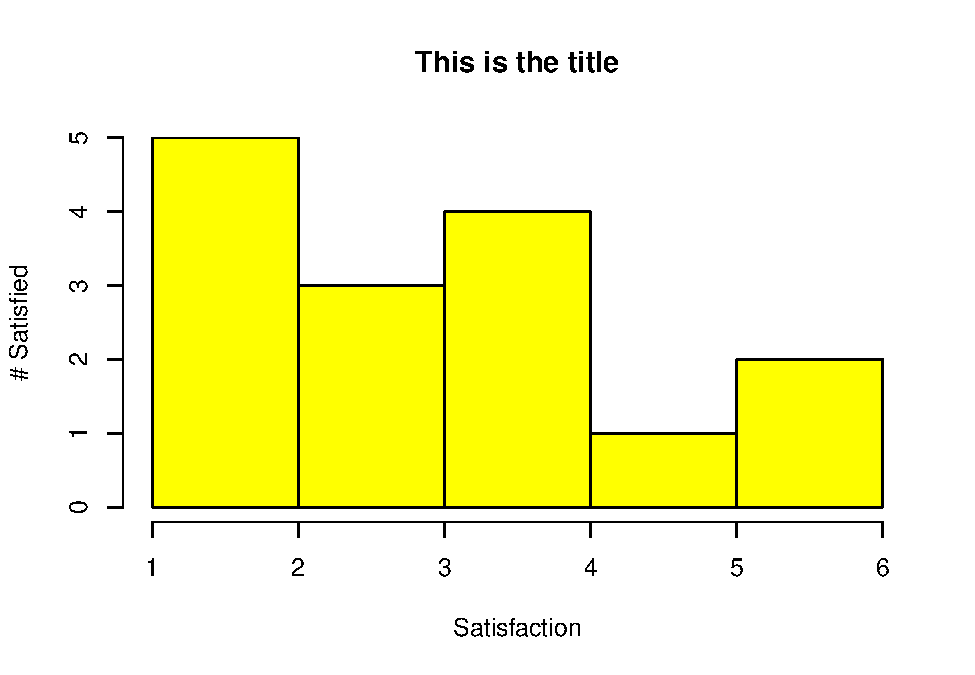
\includegraphics{3_StatisticsTerms_files/figure-latex/unnamed-chunk-2-1.pdf}

\hypertarget{barplot}{%
\subsubsection{Barplot}\label{barplot}}

\begin{Shaded}
\begin{Highlighting}[]
\NormalTok{gamer\_survey\_data }\OtherTok{\textless{}{-}} \FunctionTok{read.csv}\NormalTok{(}\StringTok{"amalgamated\_game\_survey\_250\_2022.csv"}\NormalTok{)}
\FunctionTok{barplot}\NormalTok{(}\FunctionTok{sort}\NormalTok{(}\FunctionTok{table}\NormalTok{(gamer\_survey\_data}\SpecialCharTok{$}\NormalTok{gender), }\AttributeTok{decreasing =} \ConstantTok{FALSE}\NormalTok{),}
        \AttributeTok{main =} \StringTok{"My title"}\NormalTok{,}
        \AttributeTok{xlab =} \StringTok{"Breakdown of Age by Gender"}\NormalTok{,}
        \AttributeTok{ylab =} \StringTok{"User Number"}\NormalTok{,}
        \AttributeTok{ylim =} \FunctionTok{c}\NormalTok{(}\DecValTok{0}\NormalTok{, }\DecValTok{100}\NormalTok{),}
        \AttributeTok{col=}\FunctionTok{c}\NormalTok{(}\StringTok{"red"}\NormalTok{, }\StringTok{"coral"}\NormalTok{, }\StringTok{"blue"}\NormalTok{, }\StringTok{"yellow"}\NormalTok{))}
\end{Highlighting}
\end{Shaded}

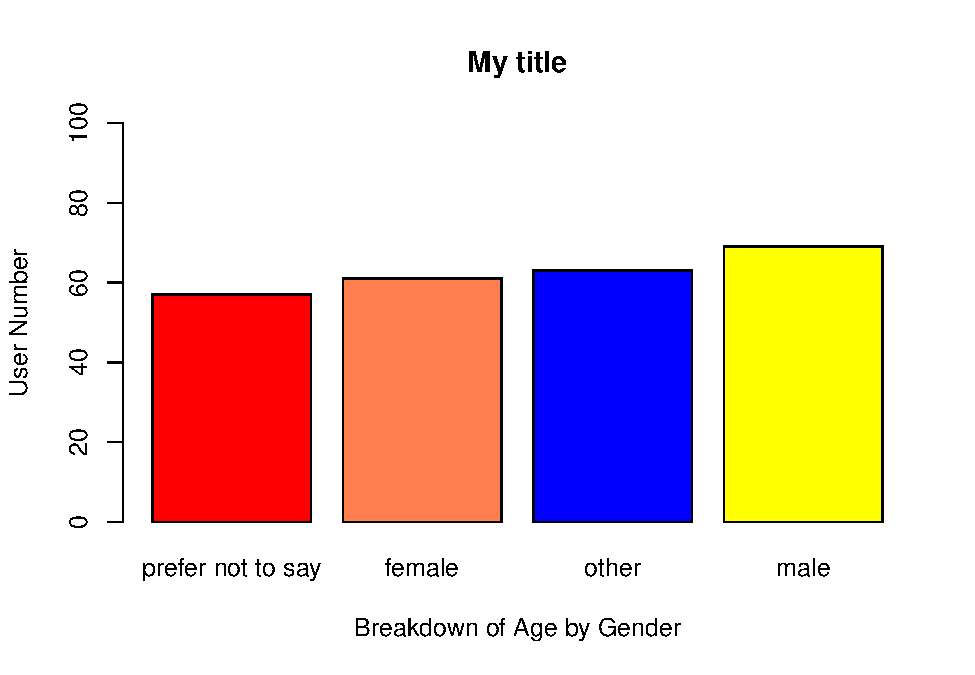
\includegraphics{3_StatisticsTerms_files/figure-latex/unnamed-chunk-3-1.pdf}

\hypertarget{boxplot}{%
\subsubsection{Boxplot}\label{boxplot}}

\hypertarget{qq-plot}{%
\subsubsection{QQ Plot}\label{qq-plot}}

\end{document}
